\documentclass[a4paper]{article}
\usepackage[warn]{mathtext}
\usepackage[utf8]{inputenc}
\usepackage[T2A]{fontenc}
\usepackage[english,russian]{babel}
\usepackage{multicol}
\usepackage{fancyhdr}
\usepackage{graphicx}
\usepackage{microtype}
\usepackage{wrapfig}
\usepackage{amsmath}
\usepackage{floatflt}
\usepackage{geometry} \geometry{verbose,a4paper,tmargin=2cm,bmargin=2cm,lmargin=1.5cm,rmargin=1.5cm}
\usepackage{float}
\usepackage{amssymb}
\usepackage{caption}
\usepackage{epsfig}
\usepackage{newunicodechar}

\begin{document}

\graphicspath{ {pic/} }
\begin{center}
    {\scshape\Large Лабораторная работа по твердотельной электронике} \par

    \

    {\huge\bfseries № 28: Исследование униполярных транзисторов с управляющим переходом} \par 

    \

    {\large Яромир Водзяновский Б04-852}
\end{center}

\

\

\begin{figure}[h]
    \begin{center}
    \begin{minipage}[h]{0.4\linewidth}
        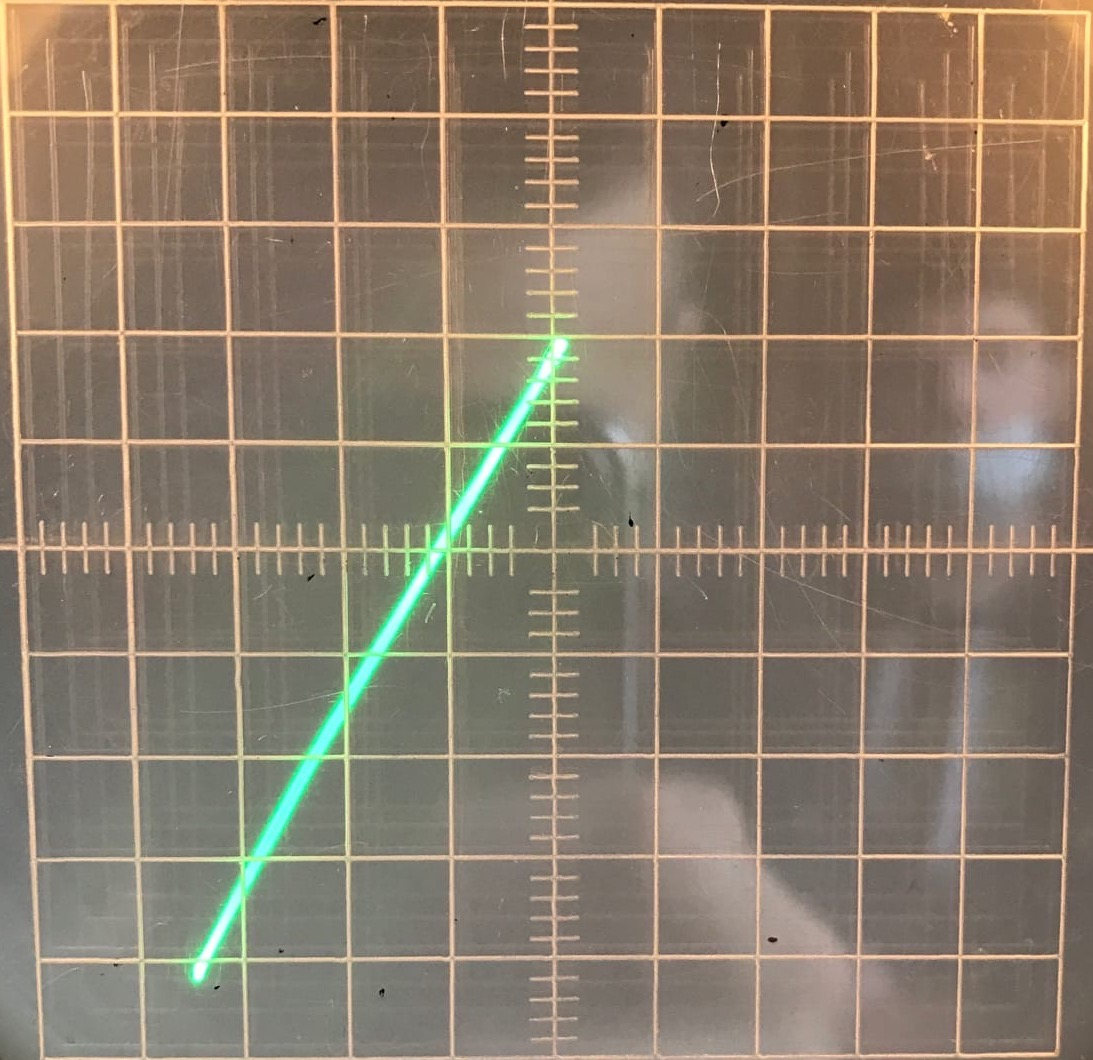
\includegraphics[width=1\linewidth]{vah1.jpg}
        \caption{ВАХ малый линейный сигнал: X = 0.02 V, Y = 0.05 mA}
        \label{vah1}
    \end{minipage}
    \hfill 
    \begin{minipage}[h]{0.4\linewidth}
        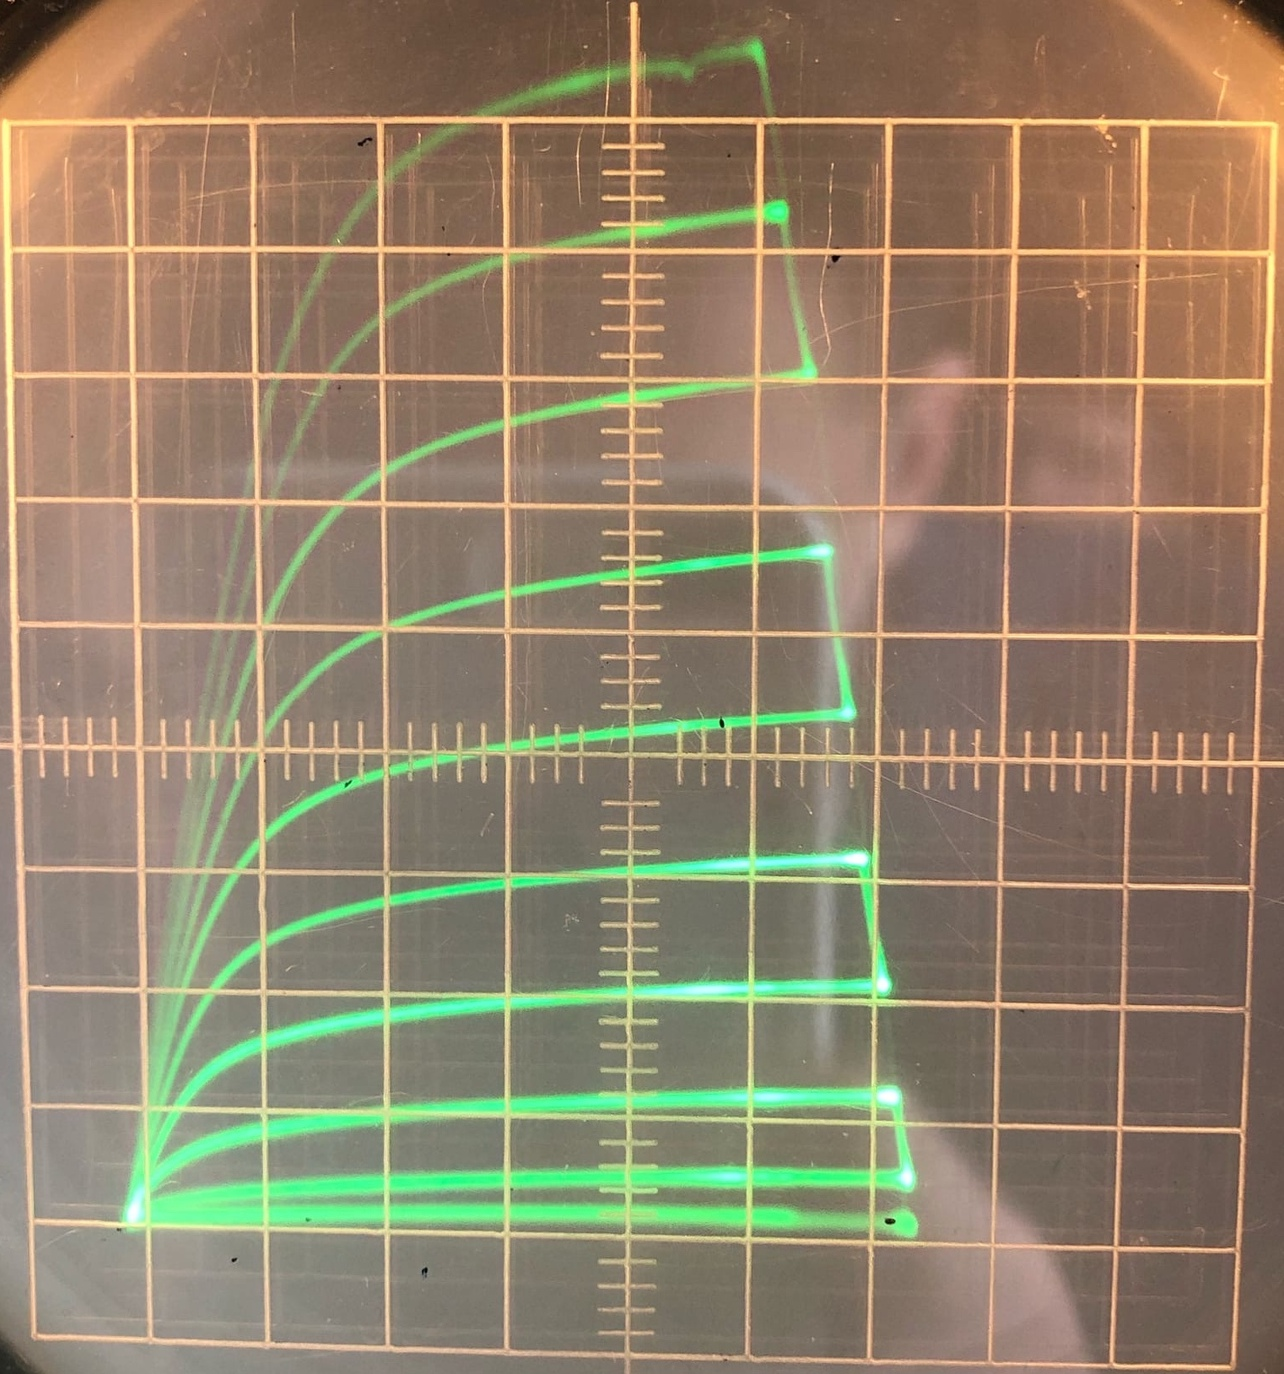
\includegraphics[width=1\linewidth]{vah2.jpg}
        \caption{ВАХ: X = 1 V, Y = 0.5 mA}
        \label{vah2}
    \end{minipage}
    \end{center}
\end{figure}

\begin{enumerate}
    \item Рассчитаем ток насыщения по формуле для диода Шоттки:
    $$I = I_s \cdot \left( e^{\frac{V}{\theta \cdot \varphi_T}} - 1 \right),$$
    положим $\theta \approx 2, \;\; \varphi_T \approx 0.026 \; V$.
    Сопротивление на данном участке (рис. \ref{vah1}) :

    \begin{center}
    \fbox{$R = 219\; Ом$ },
    \end{center}
    тогда получим:
    \begin{center}
    \fbox{$I_s \approx 0.234 \; mA$}
    \end{center}

    \item Измерим приращение тока стока. \par
    Определим напряжение запирания: 

    \begin{center}
        \fbox{$U_{зап} \approx -1.9 \; V$}
    \end{center}
    Кривизна графика в окресности точки $I_0 = 3 \; mA,\;\; U_0 = 4\; V:$
    \begin{center}
        \fbox{$S = \frac{I_{сток}}{V_{затв}} \approx 3.5 \; mA/V$}
    \end{center}

\end{enumerate}



	



\end{document}